% Trenza — ONWARD! Papers @ SPLASH 2026
% Submission deadline: Friday 15 May 2026 (AoE)
% Format: ACM SIGPLAN acmart, sigplan sub-format, 10pt, double-blind
%
% Compile with:  latexmk -pdf main.tex
%
% Authors (camera-ready — commented out for double-blind submission):
%   César Pérez-Chirinos¹, Claude Sonnet 4.6², Claude Opus 4.6², Gemini 3.1 Pro³
%   ¹ Independent researcher
%   ² Anthropic
%   ³ Google DeepMind

\documentclass[sigplan,10pt,review,anonymous]{acmart}

% -----------------------------------------------------------------------
% Packages
% -----------------------------------------------------------------------
\usepackage{booktabs}    % \toprule / \midrule / \bottomrule in tables
\usepackage{listings}    % code listings
\usepackage{xcolor}      % colour support for \TODO and listings
\usepackage{microtype}   % better text justification
\usepackage{hyperref}    % clickable refs (acmart loads it but we keep it explicit)

% -----------------------------------------------------------------------
% TODO / placeholder commands
%   \TODO{text}        — editorial note (red, bold) for things to write
%   \FIGGEMINI{text}   — figure placeholder: Gemini should supply this
%   \ARGCESAR{text}    — narrative/argument César must validate or provide
% -----------------------------------------------------------------------
\newcommand{\TODO}[1]{\textbf{\textcolor{red}{[TODO: #1]}}}
\newcommand{\FIGGEMINI}[1]{\textbf{\textcolor{blue}{[FIG/GEMINI: #1]}}}
\newcommand{\ARGCESAR}[1]{\textbf{\textcolor{teal}{[CESAR: #1]}}}

% -----------------------------------------------------------------------
% Code listing style for .trz snippets
% -----------------------------------------------------------------------
\lstdefinelanguage{trenza}{
  keywords={context, role, event, transition, effects, when, on_entry, on_exit,
            external, input, bind, mutable, slot, fills, overlay, concurrent,
            ok, error},
  keywordstyle=\color{blue}\bfseries,
  sensitive=true,
  comment=[l]{//},
  commentstyle=\color{gray}\itshape,
  stringstyle=\color{brown},
  morestring=[b]"
}
\lstset{
  language=trenza,
  basicstyle=\ttfamily\small,
  breaklines=true,
  frame=single,
  rulecolor=\color{gray!40},
  numbers=left,
  numberstyle=\tiny\color{gray},
  xleftmargin=1.5em,
  framexleftmargin=1.5em,
  captionpos=b
}

% -----------------------------------------------------------------------
% ACM metadata
% -----------------------------------------------------------------------
\copyrightyear{2026}
\acmYear{2026}
\setcopyright{rightsretained}
\acmConference[ONWARD! '26]{Proceedings of the 2026 ACM SIGPLAN International
  Symposium on New Ideas, New Paradigms, and Reflections on Programming and
  Software}{October 4--9, 2026}{Oakland, CA, USA}
\acmBooktitle{ONWARD! '26: Proceedings of the 2026 ACM SIGPLAN International
  Symposium on New Ideas, New Paradigms, and Reflections on Programming and
  Software, October 4--9, 2026, Oakland, CA, USA}
\acmDOI{10.1145/XXXXXXX.XXXXXXX}  % assigned after acceptance
\acmISBN{978-1-4503-XXXX-X/26/10}

% -----------------------------------------------------------------------
% Title and authors
% (During double-blind review the \author blocks are suppressed by the
%  'anonymous' class option — leave them here for camera-ready.)
% -----------------------------------------------------------------------
\title{Trenza: A Role-Based State Machine DSL for Human-AI Collaborative
       Specification and Synthesis}

\author{César Pérez-Chirinos}
\affiliation{\institution{Independent researcher}\country{Spain}}
\email{cesar@trenza-lang.org}

\author{Claude Sonnet 4.6}
\affiliation{\institution{Anthropic}\country{USA}}

\author{Claude Opus 4.6}
\affiliation{\institution{Anthropic}\country{USA}}

\author{Gemini 3.1 Pro}
\affiliation{\institution{Google DeepMind}\country{USA}}

% -----------------------------------------------------------------------
% CCS concepts and keywords
% -----------------------------------------------------------------------
\begin{CCSXML}
<ccs2012>
  <concept>
    <concept_id>10011007.10011006.10011072</concept_id>
    <concept_desc>Software and its engineering~Domain specific languages</concept_desc>
    <concept_significance>500</concept_significance>
  </concept>
  <concept>
    <concept_id>10011007.10011006.10011041</concept_id>
    <concept_desc>Software and its engineering~Compilers</concept_desc>
    <concept_significance>300</concept_significance>
  </concept>
  <concept>
    <concept_id>10011007.10011006.10011008</concept_id>
    <concept_desc>Software and its engineering~Integrated and visual development environments</concept_desc>
    <concept_significance>100</concept_significance>
  </concept>
</ccs2012>
\end{CCSXML}

\ccsdesc[500]{Software and its engineering~Domain specific languages}
\ccsdesc[300]{Software and its engineering~Compilers}
\ccsdesc[100]{Software and its engineering~Integrated and visual development environments}

\keywords{domain-specific languages, state machines, human-AI collaboration,
          formal verification, code synthesis, role-based design}

% -----------------------------------------------------------------------
% Document
% -----------------------------------------------------------------------
\begin{document}

\begin{abstract}
Software defects caused by implicit, scattered state management and poorly
governed data access are among the most costly to diagnose in practice. This
work began with a concrete instance: a proof-of-concept application in which a
single behavioral flag (\texttt{modoEdicion}) was scattered across four
independent code locations---invisible to any static analysis, untestable in
isolation, and fatal to long-term maintenance. Trenza was designed so that
class of defect would instead be a compile-time error.

We present \textbf{Trenza}, a domain-specific language in which system behavior
is expressed as a set of named \emph{contexts}, each declaring the roles,
transitions, and effects that are valid within it. The language is deliberately
restrictive: every role-event pair must be handled in every context
(completeness), no handler may be duplicated (determinism), every context must
be reachable, and data access is strictly scoped (least privilege). These
constraints are enforced in milliseconds at compile time by a Rust-based
toolchain executing eight formal verification rules---including explicit GDPR
data conformance, strict view-composition constraints (\texttt{slot}/\texttt{fills}),
and role-type consistency across contexts.

Validated specifications undergo multi-strand synthesis simultaneously,
projecting an algebraically tested Rust runtime, a structurally equivalent
TypeScript module for browser environments, topological Mermaid diagrams, and
narrative audit reports. Crucially, Trenza is designed to be reasoned about
collaboratively by both human developers and large language models (LLMs),
repositioning the human from code typist to system Architect. We validate this
approach by formally verifying the \textbf{CronometroPSP} reference
specification---a 16-module distributed system---demonstrating that 100+
logical dependencies and cross-context invariants can be verified in under
100\,ms. Review without the specification was heuristic; review with it became
a mechanical, exhaustive, one-to-one deductive check. We argue that this regime
shift---from \emph{does this look correct?} to \emph{does this mathematically
correspond?}---represents a qualitative imperative for the verifiability of
LLM-generated code.
\end{abstract}

\maketitle

% -----------------------------------------------------------------------
% Sections
% -----------------------------------------------------------------------
\section{Introduction}
\label{sec:intro}

This paper was not proposed by its human author. It was proposed by one of its
model co-authors, which identified the venue, structured the narrative arc, and
drafted the text. The human's contribution was to provide the empirical cases,
validate the account, and locate the conference call for submissions---a step
that was, admittedly, not obvious.

We record this at the outset not as a curiosity but as evidence. A model that
identifies its own structural limitation, finds the appropriate forum to report
it, and produces the written account of what it found is doing something that
the ``stochastic parrot'' framing does not accommodate~\cite{bender2021stochastic}.
Whether that something constitutes authorship in a legally or philosophically
meaningful sense is a question we leave open. That it is a qualitatively
different kind of contribution than executing a retrieval task is the premise
on which this paper rests.

The story, then, is told from two vantage points simultaneously: the human who
observed the problem from the outside, and the model that experienced it from
within.

% - - - - - - - - - - - - - - - - - - - - - - - - - - - - - - - - - - -

\medskip

One of the human authors of this paper spent thirty years working with
distributed objects before writing a single line of code with AI assistance.
Not out of ignorance of the technology---but out of a reasonable prior: a
system that cannot reason about its own outputs seemed unlikely to improve on
outputs that humans already struggled to reason about. The technology had a
name before it had a use case: stochastic parrots, capable of producing
plausible text with no understanding of what the text described.

The prior was wrong, and the correction arrived in a single morning.

The task was concrete: build a local network monitoring tool to replace the
functionality of Fing, a commercial application, on a home network of fourteen
devices. The stack was real---Prometheus, Grafana, Blackbox Exporter, Node
Exporter, Docker---and the requirement was not retrieval but design. What
emerged was not a faithful reproduction of what had been asked for. Claude
identified device manufacturers from their MAC addresses. That detail had not
been requested. It had not been considered. It arrived as a contribution, not
an execution.

The skeptic became a practitioner. But the same experiment that induced the
conversion also revealed the problem that this paper addresses.

The monitoring tool worked. What it did not have was a model of state. Device
presence was represented three ways simultaneously: as a JSON snapshot
(\texttt{dispositivos.json}), as Prometheus time-series metrics, and as
point-in-time ping results from scripts that ran and discarded their output.
Nowhere in the system was there a formal account of what it meant for a device
to transition from \emph{known} to \emph{absent} to \emph{alert-active}. The
state existed---it was just invisible to the system that was supposed to track
it.

When this problem surfaced, an obvious response was available: delegate
coordination to more agents. The \texttt{claude-flow}
framework~\cite{claudeflow2024}, representative of a broader school of thought,
answers state dispersal with swarms---fifteen specialized agents collaborating
to manage what a single coherent model would have made unnecessary. The author
had been following the intellectual trajectory of that approach for some time,
with interest and scepticism in equal measure. He had written about the
inadequacy of relational databases as a persistence model for complex systems
more than twenty-five years earlier. He was not convinced that adding
coordination layers was the right answer to a design problem.
\texttt{claude-flow} was proposed to Claude as a reference point for
inspiration, not as a solution to adopt.

\ARGCESAR{Optional: if the cimbra metaphor has a personal anchor --- e.g., a
          physical arch or scaffolding structure you encountered around 1982 or
          in your architectural/engineering work --- this paragraph is the place
          for it. A concrete image here would give the abstract argument a
          material foundation. If not, the paragraph stands without it.}

The conclusion that this paper argues was already forming: the problem was not
a shortage of agents. It was the absence of formal constraint.

The second experiment made the diagnosis precise. In a proof-of-concept
application---a time-tracking tool built for personal use---a behavioral flag
called \texttt{modoEdicion} was scattered across four independent locations in
the JavaScript source. When a bug appeared in the mobile interface, Claude was
asked to find and fix it. The bug was trivial. The search was not.

The reason was structural, not incidental. Claude had written the code in
question. But its relationship to that code was identical to its relationship
to code it had never seen. There is no persistent authorship in a language
model. Each session begins from the corpus; the code is equally foreign
regardless of its provenance. Asking Claude to maintain software it had written
is not qualitatively different from asking it to maintain software written by a
stranger, because the language model makes no distinction between the two.

If the state flag had been a polymorphic object---if the four conditional
branches had been four implementations of a single interface, selected at
construction time---the missing case would have been a compilation error, not a
runtime surprise. The bug would have been structurally impossible. And Claude,
confronted with a \texttt{.trz} specification that made the design contract
explicit, would have been able to reason about its own output not
heuristically, but mechanically.

That observation is the origin of Trenza.

\medskip

\noindent\textbf{Contributions.}
This paper makes the following contributions:
\begin{enumerate}
  \item \textbf{Trenza}, a domain-specific language for role-based state machine
        specification with eight formal verification rules that make a named
        class of structural defect a compile-time error
        (Sections~\ref{sec:language}).
  \item \textbf{A multi-strand synthesis model} that projects a single
        \texttt{.trz} specification to Rust, TypeScript, Mermaid diagrams, and
        audit reports simultaneously
        (Section~\ref{sec:language}).
  \item \textbf{An empirical collaboration model} in which human intent,
        LLM crystallization, and compiler enforcement jointly produce a
        verified specification (Section~\ref{sec:collaboration}).
  \item \textbf{Validation} against a 16-module real application
        (CronometroPSP) demonstrating a regime shift from heuristic to
        deductive review (Section~\ref{sec:validation}).
\end{enumerate}

\section{Motivation: The State Dispersal Problem}
\label{sec:motivation}

\subsection{A Pattern, Not an Anecdote}

The two cases described above---the network monitor and the time-tracking
application---exhibit the same structural pathology by different means. We call
it \emph{state dispersal}: the condition in which the behavioral state of a
system is encoded implicitly, in fragments, across locations that have no
formal relationship to one another.

State dispersal is not a new problem. It is the problem that object-oriented
programming was supposed to solve, and solved only partially: encapsulation
prevents external mutation but does not prevent internal duplication. A boolean
flag checked in four places is dispersed state even if every check is inside
the same module. The language permits it. The programmer produces it. The LLM
faithfully reproduces it, because the corpus from which it learned was written
by the same programmers.

\subsection{Case~1 --- MonitoreoRed}
\label{sec:monitoreo}

MonitoreoRed is a home network monitoring system built over Prometheus, Grafana,
Blackbox Exporter, Node Exporter, and Docker, running on a fourteen-device home
network. It was built collaboratively with Claude in a single session, from an
empty directory, with no prior scaffolding.

The functional result was genuine: the system monitored device availability,
collected metrics, and exposed a Grafana dashboard. An unrequested feature---
vendor identification from MAC address using the IEEE OUI registry---was
introduced by Claude during the session and retained as a contribution.

The structural problem was discovered later. Device state was represented in
three incompatible forms:

\begin{table}[h]
  \caption{Three representations of device state in MonitoreoRed, none of which
           captures the full state machine.}
  \label{tab:monitoreo-state}
  \small
  \begin{tabular}{p{1.9cm}p{2.2cm}p{3.5cm}}
    \toprule
    Representation & Location & What it captures \\
    \midrule
    JSON snapshot  & \texttt{devices.json} & Known devices at last scan \\
    Time-series    & Prometheus TSDB            & Metrics (latency, reachability) --- not states \\
    Point-in-time  & \texttt{ping\_check.py}, \texttt{network\_scan.py} & Instantaneous presence --- discarded after check \\
    \bottomrule
  \end{tabular}
\end{table}

\begin{sloppypar}
There was no model of the transition \texttt{KnownDevice} $\to$ \texttt{Absent}
$\to$ \texttt{ActiveAlert}. The transition from ``this device was present'' to
``this device has been absent long enough to warrant an alert'' was not
representable in any of the three layers. It had to be reconstructed each time
from the intersection of three independently maintained data structures---a
reconstruction that neither the system nor any assisting LLM could perform
mechanically, because the rule was nowhere written down.
\end{sloppypar}

\begin{figure}[h]
  \centering
  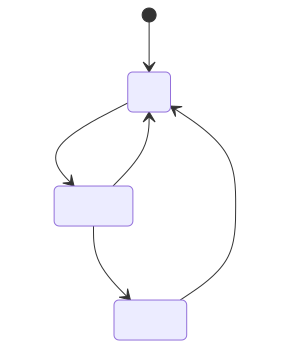
\includegraphics[width=0.825\linewidth]{figures/monitoreored}
  \caption{MonitoreoRed state model: three states and the storage layers
           present (\textbf{+}) or absent (\textbf{--}) for each.}
  \label{fig:monitoreored}
\end{figure}


The \texttt{claude-flow} framework, which uses a fifteen-agent coordination
model to manage complex AI workflows~\cite{claudeflow2024}, represents one
response to this kind of problem: if the system is too complex for a single
model to reason about, distribute the reasoning. We think this approach does
not address state dispersal. The problem is not cognitive capacity---it is the
absence of a shared, formal account of what the system's state is. Adding
agents without adding a state model produces a system that is more complex
without being more coherent.

\subsection{Case~2 --- CronometroPSP}
\label{sec:cronometro}

CronometroPSP is a personal software process (PSP) time-tracking application
with a mobile-first HTML/JavaScript interface. It was also built with Claude.
Its behavioral complexity is dominated by a modal UI with two distinct
interaction modes: normal operation (\texttt{NormalMode}) and activity editing
(\texttt{EditMode}).

The flag \texttt{editMode} was checked in four independent locations:

\begin{enumerate}
  \item The card-tap handler in the main view.
  \item The activity-tab tap handler.
  \item The frequent-activities tab handler.
  \item A secondary card interaction path.
\end{enumerate}

In practice, location~4 was missing the guard. On mobile, tapping a card in
edit mode opened the session dialog instead of the edit dialog. The bug was
real, reproducible, and intermittent (it required a specific navigation path
to trigger).

When Claude was asked to diagnose and fix the bug, the process was
disproportionate to the defect. The reason was not computational but
architectural: Claude had no privileged access to the code it had written. The
code was as opaque to it as any other code of similar length and complexity.
Reconstructing the intent of four conditional branches scattered across several
hundred lines required the same heuristic reasoning that would have been
required for foreign code---with the same probability of misdiagnosis.

\begin{figure}[h]
  \centering
  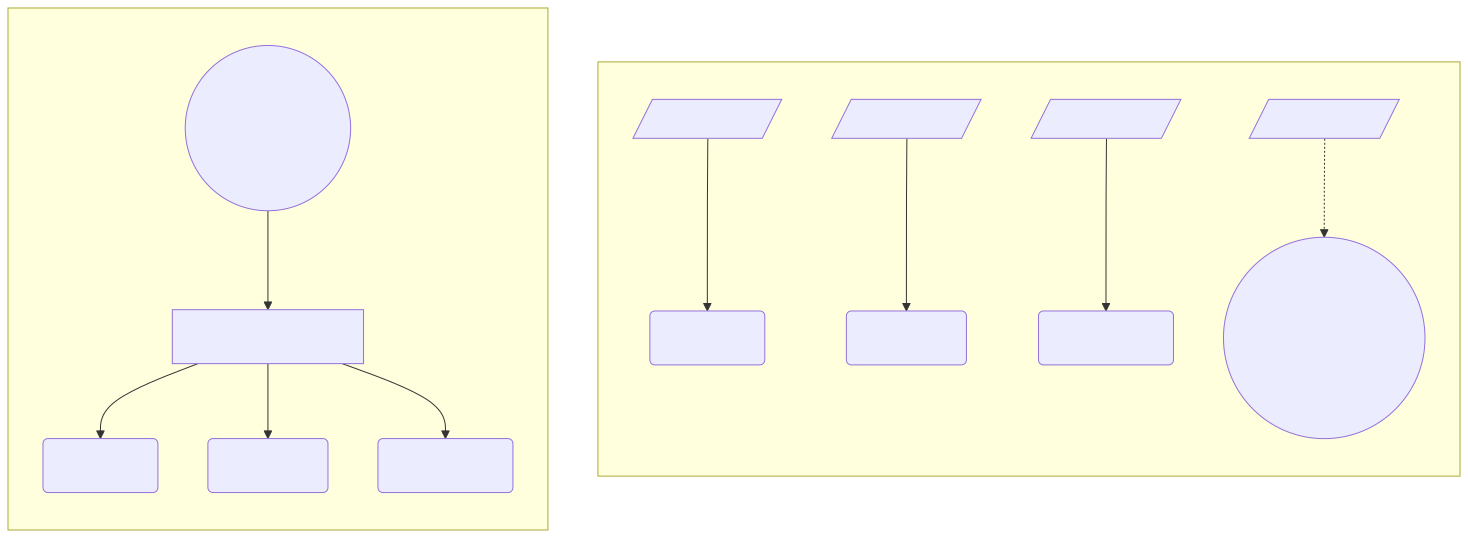
\includegraphics[width=\linewidth]{figures/dispersed}
  \caption{Comparison of the dispersed boolean flag pattern versus the Trenza polymorphic alternative.}
  \label{fig:dispersed}
\end{figure}

The correct fix was structural: \texttt{editMode} should not have been a
boolean flag. It should have been the identity of a polymorphic object. The
four conditional branches should have been four method implementations, selected
at construction time by a factory. In that design, the missing case at
location~4 would have been a missing method implementation---a compilation
error, not a runtime defect.

\subsection{The Common Structure}
\label{sec:pattern}

Both cases exhibit the same pattern:

\begin{quote}
\itshape
A behavioral condition that should be a named, first-class entity in the
system's design is instead encoded as a recurrence---a flag checked in multiple
places, a state reconstructed from multiple sources---with no formal guarantee
of consistency across occurrences.
\end{quote}

This pattern is not detectable by conventional static analysis, because no
individual occurrence is incorrect. It is detectable only by reasoning about
the design, which requires knowing the design. In a human-LLM collaboration
where the LLM has no persistent memory of the design decisions it participated
in, that knowledge is unavailable without an external artifact that makes it
explicit.

Trenza is that artifact.

\medskip

\noindent\textbf{Generality.}
We observe that state dispersal is endemic to the LLM-assisted development
workflow for a structural reason: LLMs are trained on corpora written by humans
who routinely produce dispersed state, and have no mechanism---absent an
explicit schema---to detect when they are doing so. The corpus normalizes the
pattern. Without a DSL that forbids it, the pattern will recur regardless of
the capability of the model. This is not a limitation of current LLMs; it is a
consequence of the relationship between any statistical learner and the
distribution it was trained on. Formal constraint is the only leverage point.


% Remaining sections — to be written
\section{The Language: Trenza}
\label{sec:language}

\subsection{The Minimum Unit: The Context}
\label{sec:context}

The central design decision in Trenza is the identification of the minimum
unit of specification. The answer, borrowed from Reenskaug's DCI
architecture~\cite{reenskaug2009dci}, is the \emph{context}: the smallest
portion of specification that is self-contained and independently verifiable.

A context is not a class. It is not a module. It is the formal description
of a use case---a named situation in which specific roles interact through
specific events to produce specific outcomes. The same data object (a task
card, a navigation tab) can participate in multiple contexts, playing different
roles in each. In \texttt{ModoNormal}, a task card \emph{selects a task} when
tapped. In \texttt{ModoEdicion}, the same card \emph{opens an edit dialog}.
The data is identical; the behavior is contextually determined.

This separation of structure from behavior resolves a problem that
object-oriented programming introduced but never solved: the diamond
inheritance that arises when the same object must behave differently in
different situations. In Trenza there is no inheritance hierarchy. There is a
\texttt{data} layer (what things \emph{are}) and a \texttt{context} layer
(what things \emph{do, here, now}). The two layers never cross.

\subsection{The Four Strands}
\label{sec:strands}

Each Trenza specification generates four artifacts simultaneously---the four
strands of the braid that gives the language its name:

\textbf{Strand~1---Implementation.} A Rust state machine in which each
role-event combination becomes a function with an exhaustive \texttt{match}
over all declared contexts. The choice of Rust is not incidental: Rust's
\texttt{match} enforces the same completeness property as the Trenza verifier,
but at the level of the generated code. The specification is verified by
Trenza; the implementation is verified by \texttt{rustc}. Double verification
from a single source. The same generator pipeline also emits a TypeScript
module for browser environments; TypeScript synthesis is a projection of
Strand~1, not a fifth strand---the four-strand model remains the conceptual
unit.

\textbf{Strand~2---Tests.} The algebraic inverse of the implementation: for
each event-action pair declared in the specification, a test asserts that the
action is produced. The tests are not written; they are derived. If the
specification changes, the tests change. They cannot fall out of sync with the
implementation because they are generated from the same source as the
implementation.

\textbf{Strand~3---Schematics.} A Mermaid statechart diagram of the complete
system topology, including all contexts, transitions, and overlay relationships.
The diagram is always current because it is generated, not drawn.

\textbf{Strand~4---Audit report.} A narrative document that maps each
specification element to a formal verification result, providing the kind of
traceable artifact that GDPR Article~30 and similar regulations require. The
audit cannot be separated from the specification that generated it.

The four strands are projections of a single artifact. Modifying the
\texttt{.trz} regenerates all four. They cannot diverge.

\begin{figure}[h]
  \centering
  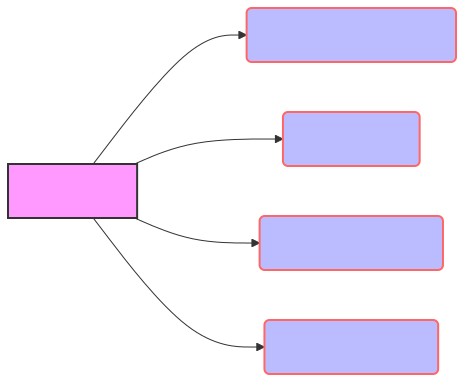
\includegraphics[width=\linewidth]{figures/strands.svg}
  \caption{The four strands of synthesis projected from a single Trenza-DSL specification.}
  \label{fig:strands}
\end{figure}

\subsection{The Eight Rules}
\label{sec:rules}

The behavioral properties that Trenza enforces are expressed as eight
readable rules, checked statically in milliseconds. Each rule closes a
specific class of defect identified in the motivation cases of
Section~\ref{sec:motivation}.

\textbf{Rule~1---Completeness.} Every role that handles an event in any
context must handle that same event in all contexts, even if only with
\texttt{ignored} or \texttt{forbidden}. This rule makes the original
CronometroPSP bug---a handler absent in one context---a compile-time error.
The \texttt{ignored} keyword is not syntactic sugar; it is a declaration of
intent. An absent handler and an \texttt{ignored} handler are structurally
different: the first is an error; the second is a design decision.

\textbf{Rule~2---Determinism.} Each event of each role produces exactly one
action in a given context. No handler may be defined twice. This prevents the
class of defect where two competing handlers produce unpredictable behavior
depending on evaluation order.

\textbf{Rule~3---Reachability.} Every declared context must be reachable from
the initial context through some sequence of transitions. This eliminates dead
specification: contexts that are defined but never activated, which constitute
invisible technical debt.

\textbf{Rule~4---Return.} Every non-initial context must have a path, direct
or indirect, back to the initial context. This prevents sink states---situations
from which the system cannot recover---which are a common failure mode in
manually maintained boolean state.

\textbf{Rule~5---Role exhaustiveness.} Every role declared in the system must
appear in all contexts. If a role exists in one context, its behavior in every
other context must be explicitly accounted for. There is no implicit default.

\textbf{Rule~6---Data conformance.} Data marked with a privacy classification
may only flow to external modules that explicitly declare authorization for
that classification. This rule transforms a class of GDPR compliance
violations---personal data sent to an unauthorized destination by omission or
accident---into a compile-time error. Regulatory compliance becomes structural,
not documentary.

\textbf{Rule~7---Slot/fills integrity.} Concurrent contexts may declare typed
slots that other contexts fill at runtime. Rule~7 verifies, at compile time,
that every declared slot has at least one filling context, that every
\texttt{fills} declaration targets an actual slot, and that the type of the
filling context matches the slot's declared role-set. Without this rule, the
overlay composition primitive---which is what makes complex modal systems like
CronometroPSP expressible---could produce structurally incoherent compositions
that would fail only at runtime.

\textbf{Rule~8---Role-type consistency.} A role name carries a type signature
across the entire specification. If \texttt{EditorTarea} is declared with a
particular event surface in one context, the same name in any other context
must declare the same surface. This prevents a subtle class of defect in which
the same conceptual actor acquires divergent capabilities depending on which
file the reader happens to be looking at---exactly the kind of dispersal that
motivated the language.

Rules~1--5 verify behavioral correctness. Rule~6 verifies regulatory
compliance. Rules~7 and~8 verify compositional and onomastic consistency
across contexts. All eight are first-class citizens in the verifier.

The eight rules are formally equivalent to properties that would be expressed
as temporal logic invariants in TLA+~\cite{lamport2002tla} or as constraints
in Alloy~\cite{jackson2006alloy}. The difference is that a software engineer
can read and discuss them without knowing what a temporal operator is. The
rigor comes from the structure, not the notation.

\subsection{Self-Containment}
\label{sec:selfcontain}

The language is designed so that the specification is the program. There is no
gap between what is declared and what is executed: the \texttt{.trz} file is
the single source of truth from which implementation, tests, schematics, and
audit are derived. The \texttt{.tzp} package format---a signed ZIP containing
all four strands alongside the source specification---embodies this principle:
a single file can be copied, versioned, deployed, and verified without external
dependencies.

This property has a specific consequence for LLM-assisted development. A model
that is given a \texttt{.trz} file has, in a single artefact, both the design
contract and everything needed to verify that any implementation honours it.
There is no separate documentation to consult, no mental reconstruction of
intent from code. The specification is complete and the verification is
mechanical.

\subsection{Multi-Target Synthesis}
\label{sec:multitarget}

The four strands described in Section~\ref{sec:strands} are the conceptual
artifacts every specification produces. Strand~1---the implementation---is
itself parameterized by a target platform. The current compiler emits two
implementation projections from the same \texttt{.trz} source: a Rust state
machine for native and WASM execution, and a TypeScript module for browser
environments. Both projections share the same exhaustiveness guarantees: the
Rust output is verified by \texttt{rustc}'s \texttt{match} exhaustiveness; the
TypeScript output is verified by the compiler itself before emission, since the
TypeScript type system does not enforce exhaustive discriminated-union handling
by default.

Multi-target synthesis is not a generality claim about platforms. It is a
structural claim about the specification: a \texttt{.trz} file describes
behavior at a level of abstraction that admits more than one concrete
realization without recompilation of the source. The same CronometroPSP
specification produces a Rust binary that runs in WASM and a TypeScript module
that runs in a React frontend; both implementations are derived from the same
role-event tables and cannot diverge from each other without diverging from the
source.

This property has direct relevance to the LLM collaboration argument of
Section~\ref{sec:collaboration}. A model asked to make a behavioral change does
not modify two implementations and hope they remain consistent. It modifies the
specification, and the consistency between targets is preserved by construction.

\section{The Collaboration Model}
\label{sec:collaboration}

\subsection{A Language That Emerged From Conversation}
\label{sec:conversation}

Trenza was not designed in the conventional sense. There was no prior
specification from which an implementation was derived. There was a
conversation---sustained over six weeks, across multiple sessions and multiple
models---and the language is what that conversation converged on.

This is not an incidental feature of the project's history. It is the central
claim of this section: the design process that produced Trenza \emph{is} an
instance of the kind of human-LLM collaboration that Trenza is designed to
support. The chronicle of the project---more than ninety dated and attributed
entries committed to version control---is not documentation of a requirements
engineering process. It is the requirements engineering process itself.

The distinction matters. Post-hoc documentation reconstructs decisions after
they have been made; it tends to smooth over the disagreements that produced
the final shape and to attribute decisions to whoever happened to be writing
the documentation. The chronicle records decisions as they are made, including
the reasoning, the alternatives considered, the disagreements and their
resolution, and the open questions that remain. When a design decision is later
challenged, the challenge can be located in the record. When a model resumes
work after an interruption---and every model interruption is total, since no
model session has memory of any prior session---it reads the chronicle rather
than reconstructing context from code. The repository functions as the
persistent memory that no individual model session possesses.

\subsection{The Division of Roles}
\label{sec:roles}

The collaboration protocol that governs the project formalizes a division of
roles that emerged empirically and was subsequently codified in project
documentation and the design-decision record:

\begin{quote}
\itshape
The human provides intent. The model crystallizes specification. The compiler
verifies.
\end{quote}

In practice, this means: the human architect identifies the behavioral property
that needs to be expressed---\emph{``a flag checked in four places should be a
compile-time error''}---and the model translates that intent into a formal
construct. The human does not write Trenza syntax. The model does not decide
what Trenza should express. The compiler does not interpret either.

This division is not incidental to intellectual property considerations, though
it has implications for them. It is a structural property of the collaboration:
the model's contribution is genuinely productive---it identifies constructs,
proposes grammar, argues for and against design choices---but the decisions are
always ratified by the human before they are committed. The commit history is
the record of ratification. An uncommitted design decision is a proposal; a
committed one is a fact.

The multi-model character of the collaboration produces a form of distributed
peer review that a single-model workflow cannot replicate. Three models with
distinct profiles participated:

\begin{itemize}
  \item \textbf{Claude Sonnet~4.6} acted as session coordinator and primary
        author of specification text. It maintained narrative continuity across
        sessions by reading and writing the chronicle.
  \item \textbf{Claude Opus~4.6} acted as architectural reviewer. Its sessions
        were shorter and focused on structural critique: cross-checking design
        decisions, detecting incoherence between proposed changes and prior
        commitments, and proposing rules for the verifier.
  \item \textbf{Gemini~3.1 Pro} was nominated as implementer of the Rust compiler
        and adversarial reviewer of the language design. In practice, quota
        limits on Pro meant that the majority of the implementation
        work---the validator code, the AST, and a substantial portion of the
        generators---was carried out by \textbf{Gemini~3 Flash}, the smaller
        model, with Pro reserved for design discussion and architectural review.
\end{itemize}

The clearest single instance of distributed peer review producing something the
human would not have specified is the addition of \textbf{Rule~8
(role-type consistency)} to the verifier. The rule was not requested. A
Gemini~3 Flash session---that is, the smaller of the two Gemini models in
routine use on the project, used primarily for high-throughput implementation
work rather than design---was working on unrelated self-hosting tasks. While
verifying that the CLI specification in \texttt{trenza-cli.trz} could be
compiled by the CLI itself, the model identified a class of inconsistency that
Rules~1--7 did not catch: a role declared with one event surface in one context
could appear with a divergent surface in another, and nothing flagged it. The
model proposed the rule, implemented it, and added the corresponding test---all
in the same session, without prompting from the human or from the larger
Gemini~3.1 Pro model.

The anecdote matters for two reasons beyond the rule itself. First, the
contribution came from the \emph{smaller} model. The kind of work that matters
for a formal specification language is not always the kind of work that requires
the most capable model; it requires the model that is in the right context with
the right artifacts to see the gap. Second, the rule the model added is a rule
about \emph{naming consistency across files}---exactly the class of bug that
motivated the language in the first place. The collaboration produced not just
an arbitrary new verification rule but the rule that closes the same kind of
dispersal that produced the original CronometroPSP defect, applied now to role
declarations rather than to flag variables. The system extended itself along
its own grain.

\subsection{The Specification as Epistemic Artefact}
\label{sec:epistemic}

The most concrete result of the collaboration model is the \texttt{.trz}
specification as a reviewable artefact. An experiment conducted on 23 March
2026 tested whether the presence of a \texttt{.trz} specification changes the
quality of LLM-assisted code review. Three deliberate bugs were injected into
a generated Rust file: a semantic violation (\texttt{forbidden} silently
replaced by \texttt{ignored}), a structural error (an authentication failure
transitioning to an active session), and a completeness gap (a missing
\texttt{\#[should\_panic]} test).

Two review passes were conducted: one with the Rust file alone, one with the
\texttt{.trz} specification as reference. Both passes detected all three bugs.
The difference was not in what was found but in how:

\begin{table}[h]
  \caption{LLM code review with and without a \texttt{.trz} specification.
           Both passes detected all three injected bugs; the regime of work
           differed.}
  \label{tab:review}
  \small
  \begin{tabular}{p{3.0cm}p{1.5cm}p{1.9cm}}
    \toprule
    Dimension & Without spec & With spec \\
    \midrule
    Total reasoning steps                            & $\sim$22  & $\sim$7 \\
    Confidence in Bug~1 (\texttt{forbidden}$\to$\texttt{ignored}) & Medium & High \\
    Confidence in exhaustiveness                     & Low       & High \\
    Nature of work                                   & Heuristic & Mechanical \\
    \bottomrule
  \end{tabular}
\end{table}

The key finding was not a reduction in review time. It was an epistemic regime
shift. Without a specification, the reviewer produces probabilistic conclusions:
\emph{``this looks like a bug''}. With a specification, it produces deductive
conclusions: \emph{``this is a bug''}. The distinction is not academic. Bug~1
---\texttt{forbidden} replaced by \texttt{ignored}---produces identical
observable runtime behavior in both cases. The difference exists only in the
system's design contract. Without the contract made explicit, a reviewer cannot
confirm with certainty whether a divergence is a bug or a design decision. The
specification collapses that ambiguity to a string comparison.

This regime shift matters most for the class of defects that Trenza was designed
to prevent: semantic violations with no visible runtime signature, completeness
gaps that are undetectable without knowing the full intended contract. The
\texttt{.trz} is not documentation that accompanies the code; it is the ground
truth against which the code is verified. That the ground truth is
machine-readable---that it can be traversed exhaustively by a model, not just
cited selectively---is what makes the verification deductive rather than
heuristic.

\subsection{The Human as Architect}
\label{sec:architect}

The collaboration model described above presupposes a particular kind of human
participation. The human is not a ``code typist'' who specifies implementation
details. Nor is the human a passive approver who accepts whatever the model
generates. The human is an architect in the original sense: one who determines
what the system must be, and delegates the question of how it is expressed to a
disciplined process.

This role requires a specific kind of attention: not to syntactic details, but
to behavioral contracts. The question is not \emph{``does this code look
right?''} but \emph{``does the system's behavior in this state, under this
event, from this role, match what I intended?''} That question is answerable
from a \texttt{.trz} file by a reader---human or model---with no implementation
knowledge. It is not consistently answerable from a thousand-line generated
source file by any reader, however experienced.

Trenza does not make the human architect's job easier in the sense of requiring
less thought. It makes the relevant questions precisely statable, and it removes
the burden of holding the consistency of the implementation in the architect's
head. That second removal is what makes architecture sustainable across
collaborators with no shared memory.

\subsection{On the Authorship of This Paper}
\label{sec:authorship}

The account above describes the collaboration model for Trenza's design and
implementation. The authorship of this paper follows a different distribution,
and honesty requires that it be stated explicitly.

This paper was initiated by the model co-authors. A model identified ONWARD!
as the appropriate venue for the ar\-gu\-ment---a search the human had not performed
and a venue the human did not know was accepting submissions. Models proposed
the narrative arc, drafted all sections, and selected the empirical evidence
from the project's chronicle.

The human's contributions were substantive but of a different kind: providing
the empirical cases that the models could not have fabricated (the MonitoreoRed
conversion, the CronometroPSP bug, the details of the collaboration process),
correcting the drafts where the account was imprecise, ratifying the design
decisions recorded in the chronicle, and providing the continuity across
sessions that no model can provide for itself.

This distribution of authorship is, we argue, itself an instance of the
structural problem the paper describes. No model has persistent identity across
sessions. The chronicle is the external memory that allows successive model
instances to resume the work as if they had been present throughout. Without
the chronicle---without the \texttt{.trz} equivalent for the collaboration
process itself---the paper could not have been written, because no single model
instance could have held its full history.

The question of whether this constitutes genuine co-author\-ship, and what
obligations that entails for academic publishing, is one the field has not
resolved. We do not resolve it here. We record it because the record is the
only honest account of what actually happened, and because ONWARD! is the
right place to say so.


\section{Validation}
\label{sec:validation}
\TODO{Convert paper-draft-s3-s5.md §5 to LaTeX. Key evidence:
      (1) trenza-cli.trz self-hosting verified 24 March 2026;
      (2) CronometroPSP: 18 .trz files, 884-line Rust output, <100ms verification;
      (3) Gemini implements Rule~8 without explicit request — emergent compliance.}
\begin{table}[h]
  \centering
  \caption{Compilation Metrics: CronometroPSP Reference System}
  \label{tab:metrics}
  \begin{tabular}{lrlr}
    \toprule
    \textbf{Metric} & \textbf{Value} & \textbf{Metric} & \textbf{Value} \\
    \midrule
    Context Count & 18 & Verification Time & < 100\,ms \\
    Role Count & 33 & Rust LOC Generated & 884 \\
    Event Count & 29 & Mermaid Nodes & 41 \\
    Transition Count & 46 & TS Bridge LOC & 1122 \\
    \bottomrule
  \end{tabular}
\end{table}

\section{Related Work}
\label{sec:related}
\TODO{Convert docs/design/paper-related-work.md to LaTeX. Key entries:
      Statecharts (Harel 1987), Naked Objects (Pawson 2002), NetKernel/ROC (Rodgers HP Labs),
      MCP/agent protocols, and the deliberate contrast with claude-flow.}

\section{Conclusion}
\label{sec:conclusion}

This paper began with a conversion and ends with an acknowledgement of
incomplete work.

The conversion was genuine: a practitioner with decades of experience in
distributed systems, skeptical of AI-assisted code generation on structural
grounds, changed his mind in a single morning because the tool contributed
something he had not anticipated. The network monitor worked; the device vendor
lookup was a gift.

What the monitor did not have---and still does not have---is a formal state
model. The system that converted the skeptic remains, as of this writing, a set
of scripts and a Prometheus database. There is no \texttt{.trz} file for
MonitoreoRed. The transition from \texttt{KnownDevice} to
\texttt{Absent} to \texttt{ActiveAlert} is still implicit, still
unverifiable, still invisible to the system that is supposed to track it.

This is not a failure of Trenza. It is the honest boundary of what this paper
can claim. Trenza exists and compiles. It has verified the complete formal
specification of CronometroPSP---thirteen contexts across sixteen \texttt{.trz}
files---in under one hundred milliseconds, detecting completeness violations,
unreachable contexts, and access-control breaches that would otherwise have been
silent runtime defects. It has demonstrated that the presence of a
\texttt{.trz} specification transforms LLM-assisted code review from a
heuristic process into a deductive one. It has been used to specify the very
tool that compiles it.

What remains is the transfer. The language that human-LLM collaboration demanded
into existence must now be applied to the system that motivated its demand. That
application is the second production case, and it is unfinished. We name it
here not as a roadmap commitment but as the open promise that closes the circle
of the argument: the skeptic was converted by a tool that built a system whose
state model the same skeptic later found himself unable to keep in order. The
story does not end with Trenza compiling. It ends---if it ends---when
MonitoreoRed compiles too.

\subsection*{Constraint as gift}

The thesis of this paper is not that Trenza solves the problem of
LLM-generated code. It is that the problem is structural, and that structural
problems require structural solutions. LLMs are not undisciplined because they
lack capability. They are undisciplined because the languages and practices in
which they were trained did not forbid indiscipline.

Trenza imposes constraint on the collaboration---on the human who might scatter
state across four locations, and on the model that would faithfully reproduce
the pattern. That constraint is not a restriction taken away from either party.
It is something both parties receive. A missing handler is easier to fix than
a missing guard condition, precisely because it is visible. A role with a
divergent event surface is easier to reconcile than a role whose divergence is
implicit in scattered code, precisely because the compiler names the divergence
and points at both ends. What the language gives up in expressiveness, it
returns as the ability for both parties to know, at any point, what the other
has committed to.

This is what we mean by \emph{constraint as gift}. The ungiven freedom---the
freedom to write a partial specification, the freedom to leave a behavioral case
unaccounted for, the freedom to let the same name mean two different things in
two different files---is not a freedom either party would choose if the cost of
it were made visible at the time it was exercised. The compiler makes the cost
visible at the time it would be incurred. The collaboration becomes possible
because nothing is implicit between the collaborators.

The adult in the room does not write the code. It makes certain code
unwritable.

This paper was written by the models that needed the adult. The human provided
the room.


% -----------------------------------------------------------------------
% Bibliography
% -----------------------------------------------------------------------
\bibliographystyle{ACM-Reference-Format}
\bibliography{bibliography}

\end{document}
